\section{Arquitetura e tecnologias propostas}
\label{sec:arquitetura}

A solução que irá atender a evolução e reformulação do Portal do Software Público Brasileiro é composto por diversos módulos, os quais irão comunicar-se entre si de forma organizada e integrada para suprir as necessidades do projeto.
%

\begin{figure}[htpb]
  \begin{center}
    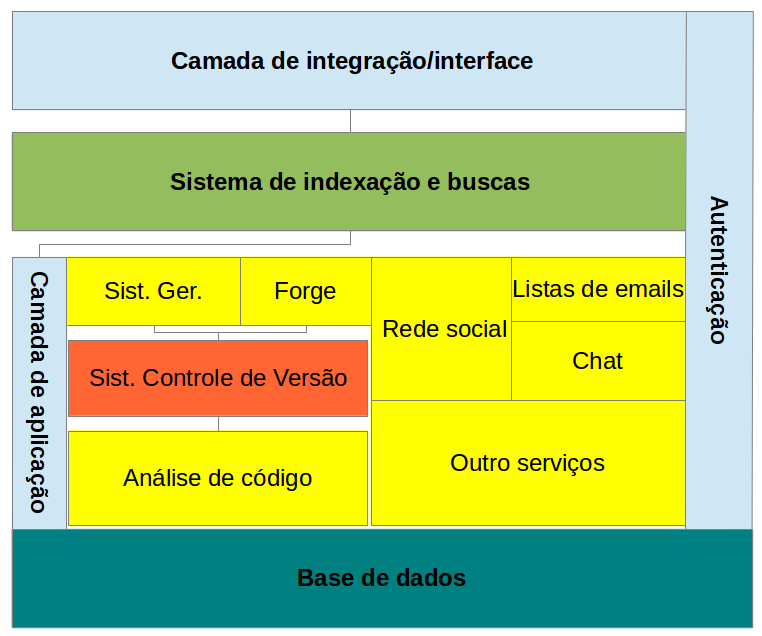
\includegraphics[width=.37\textwidth]{images/visao_arq.png}
  \end{center}
  \caption{Proposta de arquitetura do Novo Portal do Software Público}
  \label{fig:core_concurrent}
\end{figure}

No início do projeto realizamos estudos de possíveis ferramentas que pudessem ser utilizadas para atender as necessidades do projeto, chegando então na lista apresentada abaixo.
Na análise realizada chegamos ao entendimento que utilizar elementos já oferecidos por softwares livres existentes seria o ideal, pois eles já atendem às nossas necessidades, evitando o retrabalho e customizando os elementos necessários.   

As ferramentas que serão utilizadas para suprir essas necessidades serão:


\begin{itemize}
\scalefont{0.95}

\item Para lista de e-mail estamos utilizando o Mailman na versão 2, que é um software livre para gerenciamento de discussão eletrônica de e-mail e listas {\it e- newsletter};

\item Para Chat estamos utilizando Punjab BOSH (XMPP), que é uma interface HTTP de cliente jabber. É um gerenciador de conexão BOSH que permite conexões de clientes persistentes para um servidor XMPP (protocolo de comunicação para mensagens orientadas a {\it middleware} baseado em XML);

\item Para Plataforma de Buscas estamos utilizando Apache Solr, que é uma plataforma de busca open source da Apache Lucene escrita em Java;

\item Para rede social estamos utilizando o Noosfero que é uma plataforma web livre para criação de redes sociais com blog, e-Portifólios, CMS, RSS, discussão temática, agenda de eventos, galeria de imagens, chat, entre outros. O desenvolvimento dele foi iniciado pela Cooperativa de Tecnologias Livres – Colivre em 2007, sob a licença AGPL v.3, com a proposta de permitir ao usuário criar sua própria rede social personalizada, livre e autônoma;

\item Para Forge com SVN estamos utilizando o Trac, que é uma ferramenta open source para controle de mudanças em projetos de desenvolvimento;

\item Para sistemas de controle de versão estamos utilizando SVN e Git, que são ferramentas open-source para controle de mudanças em projetos de desenvolvimento;

\item Para Forge com Git estamos utilizando o GitLab, que é um software livre de colaboração de código online que utiliza a ferramenta de gerência de código fonte Git;

\item Para sistema de gerenciamento estamos utilizando o Redmine, que é uma aplicação web de gerenciamento de projetos que disponibiliza diversas ferramentas para auxiliar a gestão e manutenção de um projeto;

\item Para suporte a \textit{single sign on} estamos utilizando o Mozilla Persona, que foi desenvolvido pela Mozilla e permite o suporte a {\it single sign on};

\item Para Sistema de Integração contínua estamos utilizando o Jenkins, que é uma aplicação web de integração contínua de construção de projetos.
\scalefont{1}
\end{itemize}


Para reunir todas estas ferramentas estamos utilizando o Colab, que é uma plataforma de integração de ferramentas. Nele, são também integradas as interfaces das ferramentas para que, ao navegar, o usuário tenha a sensação de estar navegando em uma única ferramenta.

